\newpage
\section{Struktur der trainingsbezogenen Elemente des Agenten}
\label{struktur}
Um mithilfe von ML-Agents einen Agenten in Unity zu erstellen, muss dem Robotermodell ein Script hinzugefügt werden, welches von der Klasse \dq Agent\dq{} erbt. Dadurch erstellt sich die \dq Behavior Parameters\dq{} Komponente, welche in der Abbildung \ref{fig:behavior_para} zu sehen ist. In der Abbildung gibt es viele Parameter die genauer erklärt werden müssen, um den Aufbau des Agenten besser zu verstehen. Hierzu gehören die Vector Observation, die Actions und die Use Child Sensors (dt.: nutze Kind Sensoren). Auf diese wird in den Unterkapiteln eingegangen.
\begin{figure} [ht]
	\centering
	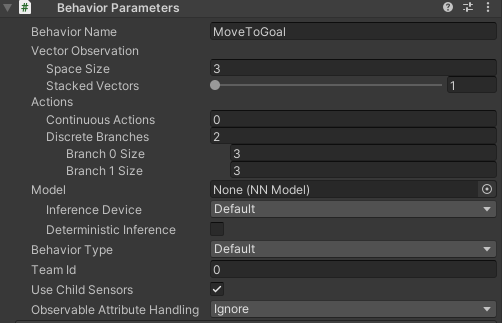
\includegraphics[width=0.6\columnwidth]{img/behavior_parameters}
	\caption[Behavior Parameter Komponente]{Die Behavior Parameters Komponente von ML-Agents.}
	\label{fig:behavior_para}
\end{figure}
\\
Die restlichen Parameter haben eine geringer Bedeutung in diesem Projekt. Der Behavior Name beschreibt den Namen des zukünftig erstellten neuronalen Netzes. 
\\Dem Model Element kann ein bereits trainiertes NN hinzugefügt werden. Daraufhin kann man die Simulation starten und des Verhalten des trainierten Modells innerhalb der Umgebung betrachten. 
\\
Das Inference Device beschreibt mit welchem Verfahren das Modell trainiert werden soll. Hier kann zwischen \dq Default\dq{}, \dq GPU\dq{}, \dq CPU\dq{} und \dq Burst\dq{} unterschieden werden. Da in früheren Projekten keine relevanten Unterschiede erkennbar waren, wurde in diesem Projekt der Default Wert verwendet. 
\\
Der Behavior Typ bestimmt darüber, ob der Agent vom Modell oder vom Nutzer gesteuert werden soll. Wenn der Default Wert ausgewählt ist, wird automatisch der Agent genutzt, falls unter Model ein trainiertes neuronales Netz hinzugefügt wurde. 
\\
Über die Team Id kann eingestellt werden, zu welchem Team ein Agent gehört. Dies wird notwendig, wenn man eine kompetitive Simulationsumgebung betrachtet, in denen Agenten gegeneinander antreten. Dazu würde beispielsweise die Soccer Umgebung von ML-Agents gehören.
\\
Über Observable Attribute Handling können weitere Beobachtungen dem Agenten hinzugefügt werden. Ein Beispiel hierfür könnten die derzeitigen Lebenspunkte eines Agenten in einem Spiel sein. Die Einstellung wurde ebenfalls nicht benutzt.
\\
Im Kapitel \ref{trainingskonfiguration} wurden die wichtigsten Punkte hinsichtlich der Betrachtung des Agenten angeschnitten. Aus den Erkenntnissen lassen sich Ableitungen für die Implementierung eines Einkaufsroboters finden. Diese werden im Folgenden ausführlich betrachtet.  

\subsection{Die Steuerung des Agenten}
Die Basis der Steuerung kann grundsätzlich in zwei Bereiche unterteilt werden. Hierzu gehört einerseits das Einlenken nach links und rechts. Andererseits die Beschleunigung vorwärts sowie rückwärts. Auf diese Basis aufbauend können dann verschiedene Stärkegrade der jeweiligen Handlung implementiert werden. Wie bei einem Auto, wo nicht nur voll nach links eingelenkt werden kann, sondern auch den Raum dazwischen. 
\\
Um dieses Verhalten zu ermöglichen, wurde initial eine Steuerung über Continuous Actions eingebaut. Dafür werden zwei verschiedene Actions benötigt, um den gesamten Bewegungsraum abdecken zu können. Bei den Continuous Actions kann der Agent bei jeder Entscheidung einen Wert zwischen minus eins und eins wählen. Diese Zahlen werden dann direkt auf die Steuerung gemappt. Beispielsweise steht der Wert minus eins dann für voll links einlenkten. Somit kann der Agent den Zwischenraum nutzen, um die Stärke seiner Beschleunigung und Lenkung zu beeinflussen. 
\\
Dies führte im Training jedoch zu sehr diskontinuierlich Verhalten. Der Agent fuhr keine zielgerichtet Linie, sondern wechselte die Richtung in jedem Entscheidungsschritt. Dadurch wirkte das Verhalten sehr unnatürlich, da der Roboter innerhalb einer Sekunde mehrmals seine Richtung komplett änderte. Diesem Problem hätte man im Code entgegenwirken können, in dem man den Grad der Richtungsänderung begrenzt. Jedoch würde dies, in Kombination mit der flacheren Lernkurve von Continuous Actions, zu deutlich längeren Trainingszeiten führen.
\\
Deswegen wechselte ich nach einiger Zeit zu den Diskrete Branches. Hier wurden wieder zwei verschiedene Actions benötigt, die ebenso für das Einlenken und Beschleunigen benutzt werden. Anders als bei den Continuous Actions kann sich der Agent in jedem Entscheidungsschritt nur zwischen drei Werten entscheiden. Null steht für nichts unternehmen, eins für links einlenken und zwei für nach rechts lenken. Gleiches gilt für die Beschleunigung. Um den Stärkegrad der jeweiligen Aktion beeinflussen zu können, wird hierfür die maximale Dauer zwischen den Entscheidungen ausgenutzt. Der Agent kann somit leicht einlenken, wenn er sich nur einmal für das Lenken entscheidet. Möchte er stärker in eine Richtung fahren, muss er sich mehrmals hintereinander dafür entscheiden. In der Abbildung \ref{fig:decision_requ} sieht man die Decision Requester Komponente von ML-Agents. Diese muss einem Agenten hinzugefügt werden, damit dieser Entscheidungen treffen kann. 
\begin{figure} [ht]
	\centering
	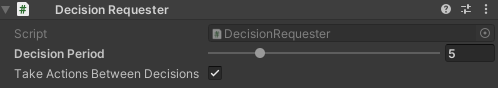
\includegraphics[width=0.6\columnwidth]{img/decision_requester}
	\caption[Behavior Parameter Komponente]{Die Behavior Parameters Komponente von ML-Agents.}
	\label{fig:decision_requ}
\end{figure}
\\
Wie man sehen kann, ist die Checkbox Take Actions Between Decision (dt.: Führe Aktionen zwischen Entscheidungen aus.) ausgewählt. Dadurch werden, wie der Name schon sagt, die Aktionen zwischen den Entscheidungen ausgeführt. Die Decision Period beschreibt, wie viele Unity Steps vergehen sollen, bis der Agent die nächste Entscheidung trifft. In diesem Beispiel beträgt die Zeit zwischen Entscheidungen 0.1 Sekunden. Dadurch wird jede getroffene Aktion 0.1 Sekunden ausgeführt. An diese Dauer kann nun die Berechnung der Steuerung abgestimmt werden, damit sie in der Simulationsumgebung möglichst natürlich wirkt.
\\
Um die Physics Engine von Unity zu verwenden, wurde dem Roboter eine Rigidbody Komponente angehangen. Die letztendlich berechneten Werte, die auf Basis der Entscheidung des Agenten beruhten, wurden dann über Funktionen des Rigidbody ausgeführt. Dem Agenten wurde zusätzlich eine gewisse Menge an Drag (dt.: Widerstand) hinzugefügt, um zu verhindern, dass er unendlich schnell wird. 

\subsection{Reward Vergabe}
Die Reward Vergabe wird entlang der Zielsetzung des Projekts modelliert. Diese wurde im Kapitel \ref{einleitung} erwähnt. Grundsätzlich soll der Einkaufsroboter möglichst schnell alle Artikel einsammeln und an einem vorgegebenen Ort abgeben. Unterstützend hierfür wird dem Agenten der kürzeste Weg zum nächsten Produkt angezeigt. Zusätzlich soll der Roboter nicht mit der Umgebung kollidieren, um Schäden an sich selbst und dem Umfeld zu verhindern.
\\
Aus dieser Zielsetzung in Kombination mit den Erkenntnissen aus dem Kapitel \ref{rewards} in dem auf die Reward Vergabe in den Beispielszenen eingegangen wurde, können nun die optimalen Rewards gebildet werden. Somit werden folgende Rewards vergeben:
\\
\begin{itemize}
	\item Existenzabzüge, um einen Anreiz zu geben, die Umgebung möglichst schnell abzuschließen
	\item kleine Belohnung beim Einsammeln von Wegpunkten 
	\item größere Belohnung für das Erreichen der Artikel
	\item sehr große Belohnung für das Erreichen des Abgabebereichs
	\item größere Abzüge bei Kollision mit den Regalen und Hindernissen
	\item kleine Abzüge beim kontinuierlichen Beistehenbleiben in einer Kollision
\end{itemize}
\noindent
\\
Die genauen Werte der Rewards veränderten sich während des Trainings. Teilweise wurden gewählte Rewards verworfen und später wieder hinzugefügt. Auf die genauen Veränderungen wird im Kapitel \ref{training_zeit} eingegangen.
\subsection{Wie sieht der Agent die Umgebung?}
\label{sensorik_agent}
In diesem Projekt wurden zwei Methoden zur Wahrnehmung der Umgebung genauer betrachtet. Hier spielen die anfangs angesprochenen Vector Observation und die Use Child Sensors eine große Rolle. 
\\
Unter Vector Observation befindet sich in der Abbildung \ref{fig:behavior_para} die Space Size (dt.: Größe des Platzes) und die Stacked Vectors (dt.: gestapelter Vektor). Space Size beschreibt die Anzahl an Werten, die an den Agenten übergeben werden. Eine Space Size von drei erlaubt, die Übergabe von drei Gleitkommawerten. Diese könnten beispielsweise die derzeitige lokale Position des Agenten im dreidimensionalen Raum darstellen. 
\\
Der Stacked Vectors Parameter beschreibt, wie viel Space Size an Daten für die nächste Entscheidung betrachtet werden soll. Bei einem Stacked Vector von eins ist nur die derzeitige Position von Bedeutung. Ein Stacked Vector von zwei übergibt die jetzige Position und die Position vor einem Zeitschritt. Damit kann der Agent möglicherweise auf Zusammenhänge schließen. 
\\
Angenommen wir betrachten das Basic Beispiel aus der Abbildung \ref{fig:basic_example}. Nur das diesmal ein Hindernis zufällig auf einer Seite vor dem Ziel platziert wird. Der Agent hat durch seine eingeschränkten Bewegungsoptionen nur die Möglichkeit, in das andere Ziel zu fahren. Würde man nur die derzeitige lokale Position des Agenten übergeben, erkennt dieser nicht, dass er nicht weiterkommt. Übergibt man aber zusätzlich die vorherige Position. Könnte der Agent darauf schließen, dass er sich zwischen dem letzten Zeitschritt und dem jetzigen nicht von der Stelle bewegt hat. Dadurch könnte er zielgerichteter die Entscheidung treffen in die andere Richtung zu fahren.
\\
Wichtig anzumerken ist, dass durch längeres Training der Agent ohne Stacked Vector trotzdem auf die Lösung kommen würde und in das andere Ziel fährt. Jedoch gilt dies nur für diese einfache sehr deterministische Umgebung. Bei Simulationen in denen sich das Umfeld in jeder Iteration stark ändert und Bewegungen im zwei oder dreidimensionalen Raum stattfinden, kann es schnell passieren, dass der Agent steckenbleibt.
\\
Die in den Beispielszenen verwendeten Vector Observation beinhalten häufig Informationen über die eigenen Parameter des Agenten und die des Ziels. Die Werte reichen aber nicht aus, um sich in einer Umgebung mit Hindernissen zurecht zu finden. Dafür sind die Use Child Sensors von Bedeutung. Damit können dem Agenten Sensoren als Kind Objekte angeheftet werden und der Agent benutzt automatisch die erhaltenen Daten. Für die Wahrnehmung der Umgebung eignen sich die Ray Perception Sensoren. Diese senden, wie in Abbildung \ref{fig:ray_sensor} zu sehen, Strahlen aus, welche bei Kontakt mit einem Objekt Daten an den Agenten weiterleiten. Hierzu gehören die Tags, welche für Objekte in der Szene ausgewählt werden können. So kann man entscheiden, worauf der Agent reagieren und was er als unterschiedliches Objekt wahrnehmen soll. 
\begin{figure} [ht]
	\centering
	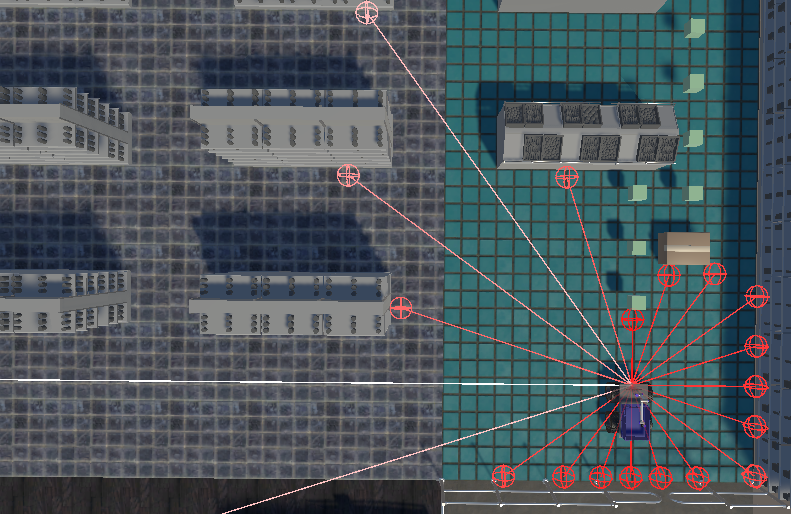
\includegraphics[width=\linewidth,height=\textheight,keepaspectratio]{img/ray_sensor_agent}
	\caption[Ray Perception Sensor in Simulation]{Ray Perception Sensor in der Simulationsumgebung. Die rot markierten Strahlen zeigen, dass diese mit einem Objekt kollidieren. Weiße Strahlen hingegen treffen auf kein Objekt.}
	\label{fig:ray_sensor}
\end{figure}
\\
Da ein Ziel war, die Fähigkeiten des Agenten in der Wirklichkeit zu verankern, wurde diese Erkennung auf das Minimum reduziert. Für dieses Projekt wurde angenommen, dass ein ausgesendeter Strahl, welcher ein Hindernis oder eine Wand trifft, immer den selben Tag zurückgibt. Die einzige Ausnahme stellen die erstellten Wegpunkte und das Ziel dar. Diese wurden jeweils mit unterschiedlichen Tags ausgestattet. Der Grund hierfür liegt darin, dass der Agent lernen soll den Hindernissen auszuweichen und den Wegpunkten zu folgen. Hätten beide denselben Tag würde er lernen, den Wegpunkten nicht zu folgen, da er den Tag voraussichtlich mit einer Bestrafung in Verbindung setzt. 
\\
Die Einstellungsmöglichkeiten des Ray Perception Sensor sind in der Abbildung \ref{fig:ray_component} zu sehen. Unter Detectable Tags (dt.: erkennbare Marken) können die Tags hinzugefügt werden, die der Sensor erkennen soll. 
\\
Rays Per Direction (dt.: Strahlen pro Richtung) beschreibt die Anzahl an Strahlen die ausgesendet werden. Dabei teilen sich die Strahlen in zwei Richtungen, wodurch sich die eingestellte Zahl verdoppelt.
\\
Die Max Ray Degrees (dt.: maximaler Strahlenwinkel) könnte man auch als Field of View (Abk.: FOV) betrachten. Eine Einstellung von 40 wurde so zu einem 80 Grad FOV führen. Die Ausrichtung der Strahlen erfolgt hierbei von einem Punkt aus in eine zusammenhängende Richtung.
\\
Den Sphere Cast Radius (frei dt.: zusätzliche Sphärenradiuserkennung) kann man am besten Anhand der Abbildung \ref{fig:ray_sensor} erklären. Hier werden anstelle eines Strahls Sphären in die jeweiligen Richtungen ausgesendet, bis diese mit einem Objekt kollidieren oder die eingestellt maximale Reichweite des Strahl (eng.: Ray Length) erreichen. Die Sphären erhöhen den Bereich in dem ein Objekt erkannt wird. Dadurch soll verhindert werden, dass ein Strahl gerade so an einem Objekt vorbeifliegt und es somit nicht erkennt.
\\
Ein weiterer wichtiger Parameter ist die Ray Layer Mask (dt.: Strahlen Ebenen Maske). Hier können bestimmte Umgebungstypen eingestellt werden, die der Sensor nicht erkennen soll. Dieser Parameter ist notwendig, um verschiedene Sensoreinstellungen zu testen. Tags, die nicht zu den Detectable Tags gehören, können zwar nicht erkannt werden, aber der Strahl kollidiert trotzdem mit dem Objekt. Wenn dem Objekt jetzt eine Maske gegeben wird, die nicht bei der Ray Layer Mask ausgewählt ist, fliegt der Strahl durch das Objekt hindurch und wird somit ignoriert. Die restlichen Werte sind selbsterklärend oder für das Training nicht weiter bedeutend.
\begin{figure} [ht]
	\centering
	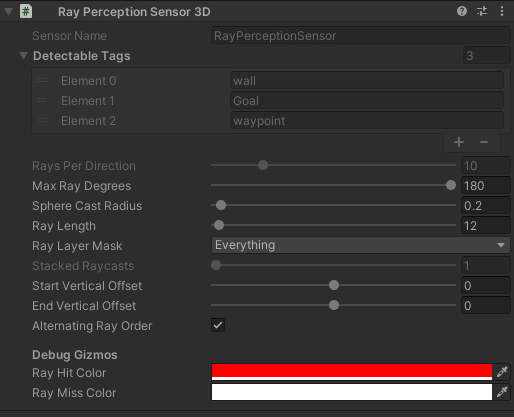
\includegraphics[width=0.6\columnwidth]{img/ray_perception_sensor_component}
	\caption[Behavior Parameter Komponente]{Die Behavior Parameters Komponente von ML-Agents.}
	\label{fig:ray_component}
\end{figure}
\\
Anders als bei Lidar Sensoren wirkt es so, als würde der Ray Perception Sensor keine Entfernungen berechnen und dem Agenten übergeben. Scheinbar wird nicht viel mehr als der erkannte Tag an den Agenten gesendet. Zwar wird in der Dokumentation\cite{ray_output} beschrieben, wie die Endposition und andere Werte ausgegeben werden können. Jedoch deuten die Ergebnisse aus dem eigenen Training daraufhin, dass der Agent diese Werte nicht erhält. Genauso wird in der Zusammenfassung zu den verschiedenen Beispielumgebungen von ML-Agents\cite{learning_environments} bei den Beispielen angegeben wie groß die Vector Observation jeweils sind. Die angegebenen Werte für die Ray Perception Sensor sind zu klein, um alle Werte aus der Dokumentation an den Agenten zu übergeben. 
\\
Der Ray Perception Sensor wird trotzdem durch unterschiedliche Einstellungen im Folgenden als vereinfachter Lidar und Ultraschallwellen Sensor verwendet. Diese Einstellungen haben sich während des Trainings immer wieder geändert, weswegen diese nicht hier sondern in dem Kapitel \ref{training_zeit} erklärt werden. 